\subsection{Bedienung des Editors}
Der Editor ist über den Text, Draw, Shape oder Image Button erreichbar. Genau wie im Reader erscheint ein Button Choose file. Je nachdem ob man auf Text, Draw, Shape oder Image geklickt hat, wird als erstes der Text-, Zeichen-, Geometrie- oder Bildeditor geöffnet.

\subsection{Textbearbeitung}
Hat man den Texteditor aufgerufen, so präsentiert sich einem der Editor in folgenden Abbildungen \ref{fig:texteditor} und \ref{fig:texteditor2}.

\begin{figure}[!htbp]
	\centering
	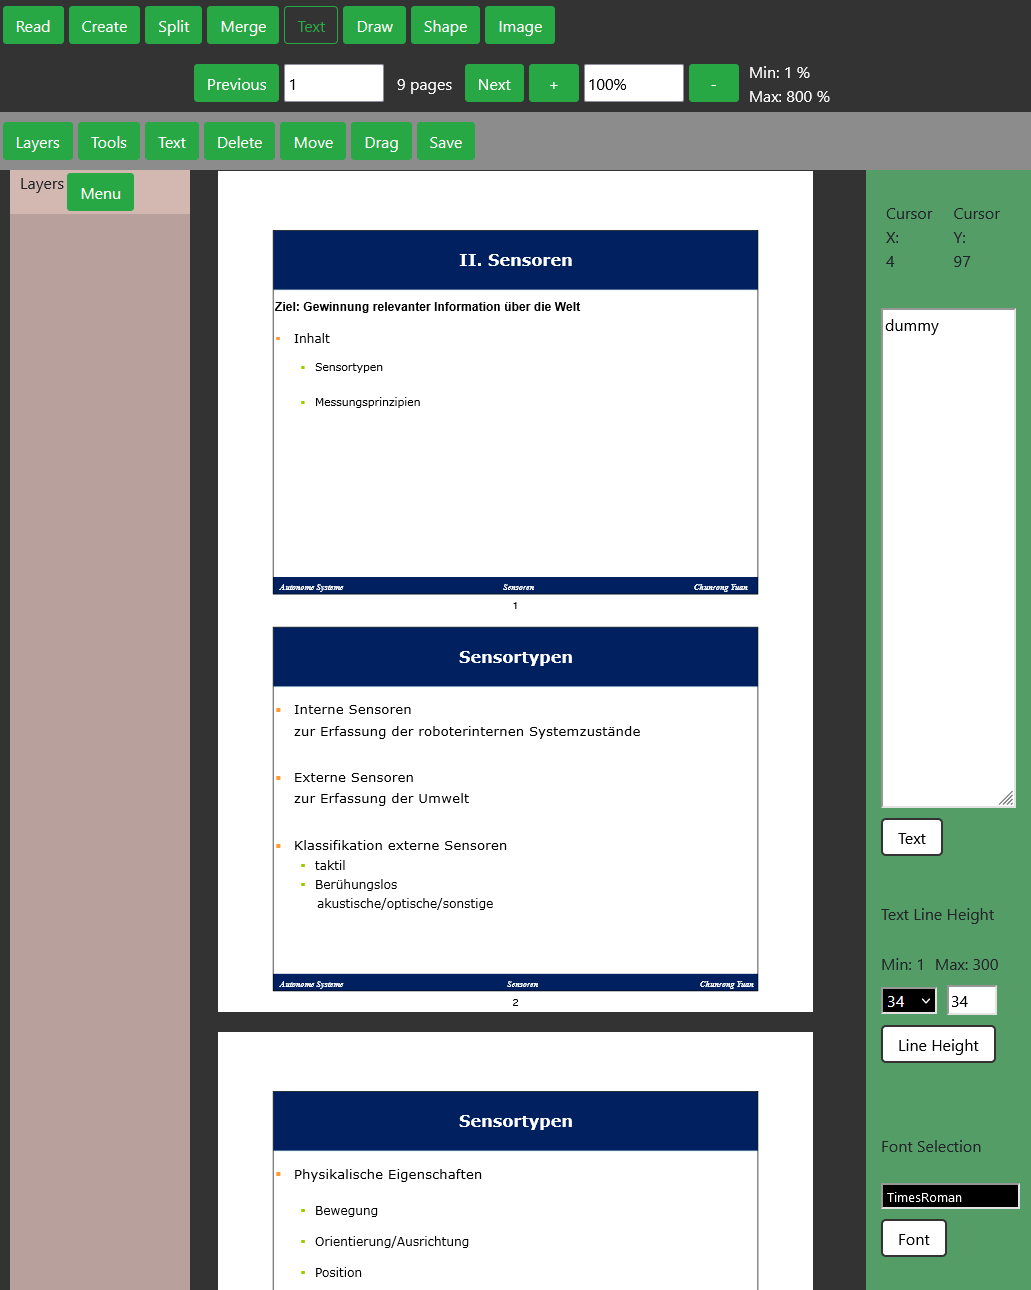
\includegraphics[width=1\textwidth]{"images/texteditor.png"}
	\caption{Startseite des Texteditors der PDF Web App}
	\label{fig:texteditor}
\end{figure}

\begin{figure}[!htbp]
	\centering
	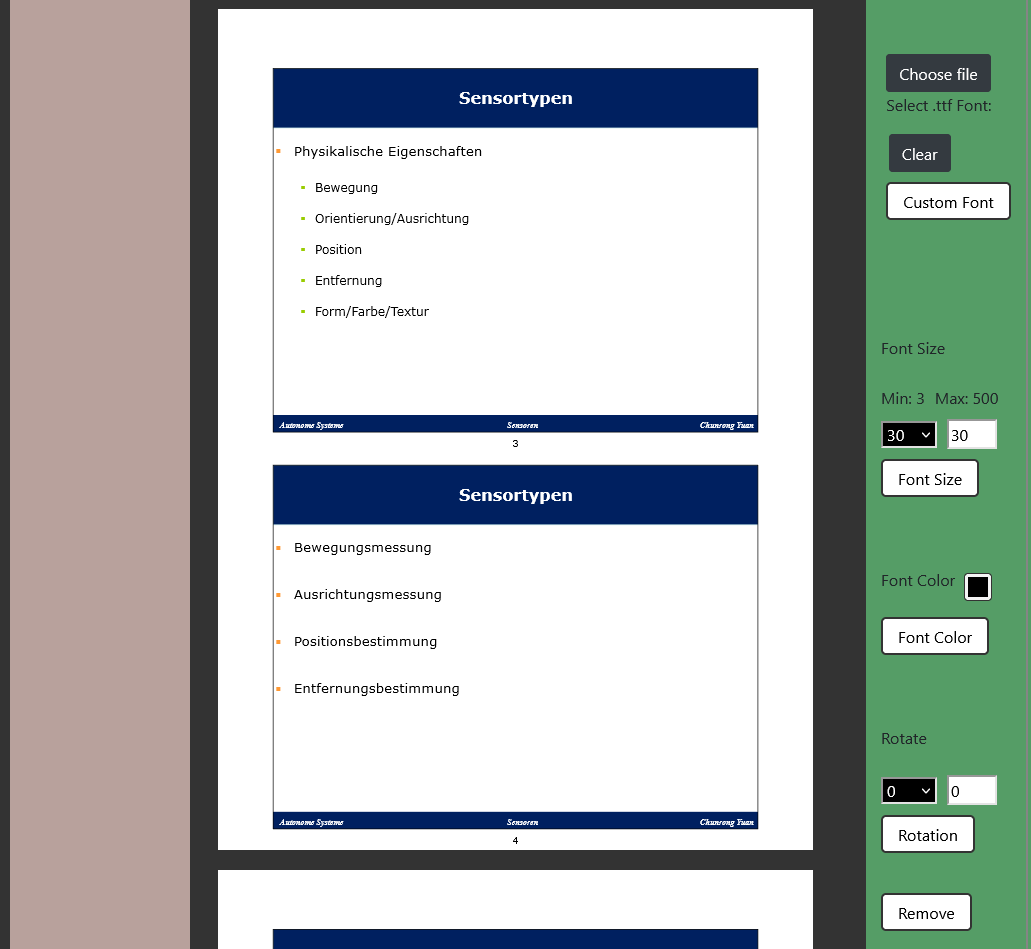
\includegraphics[width=1\textwidth]{"images/texteditor2.png"}
	\caption{Mehr Tools der Startseite des Texteditors der PDF Web App}
	\label{fig:texteditor2}
\end{figure}

Mit dem Button Text in der grauen Leiste und nachfolgendem Klick aufs geöffnete Dokument kann man einen Text hinzufügen mit dem Platzhaltertext dummy. Unter dem Text erscheint eine dunkelrote control box, auf die man alle Operationen in Tools im Box Mode anwenden kann. Der Box Mode ist standardmäßig eingestellt. Alle Operationen im rechten Tools Seitenmenü beziehen sich jeweils auf das aktuelle Editor Element und sind nur auf diesem anwendbar. Ich werde zunächst alle Operationen im Box Mode beschreiben und später auf den Layer Mode eingehen. Man kann mehrere Texte ohne erneut Text drücken zu müssen dem PDF Dokument hinzufügen. Mit dem Delete Button und nachfolgendem Klick in eine oder mehrere control boxen im Box Mode können Texte wieder gelöscht werden. Move verschiebt einzelne Texte durch mit der Maus gedrückte control box. Wenn die Maus losgelassen, nachdem die control box verschoben wurde, springt der Text an die verschobene Stelle. Im Tools Seitenmenü kann man in der textarea den Text editieren. Es werden auch Zeilenumbrüche berücksichtigt. Nachdem man den dummy Text überschrieben hat, einem Klick auf den weißen Text Button und ein oder mehrere Klicks in control boxen kann der Text angewendet werden. Alle Operationen in Tools werden genauso ausgeführt: Man macht seine Einstellung, klickt den weißen Button für die jeweilige Operation und klickt daraufhin auf ein oder mehrere Textelemente nacheinander. Darunter kann man den Zeilenabstand einstellen. Entweder verwendet man das selection menu mit voreingestellten Werten oder man gibt einen gewünschten Wert manuell ein. Falls man zuletzt das selection menu betätigt hat, überschreibt es den Wert im input field und umgekehrt. Das ist bei jeder selection menu und input field Kombination programmiert worden. Einen benutzerdefinierten Font kann man durch den Choose file Button auswählen und er erscheint in der Liste. Der zuletzt hochgeladene Font wird ausgewählt. Mittels clear kann man einen ausgewählten Font aus der Liste entfernen, was nicht heißt, dass er auch auf dem angewendeten Text entfernt wird. Die Fontgröße kann man ebenfalls wie die Zeilenhöhe mit selection menu und input field justieren. Bei der Fontfarbe klickt man auf das initial schwarze Quadrat, was die aktuelle Farbe zeigt, und es öffnet sich ein color picker Menu. Hier kann man die Farbe und Transparenz einstellen. Die Werte kann man sich in RGBA, HSLA oder HEX Format anzeigen. Mit Klick auf die beiden Pfeile wird jeweils das Format gewechselt. Als vorletzte Option kann man den Text drehen und zuletzt alle Textelemente im Dokument mit dem Remove Button entfernen.
Die Abbildung \ref{fig:texteditor3} zeigt einen modifizierten Text mit benutzerdefiniertem Font und Abbildung \ref{fig:fontcolor} zeigt den color picker für die Fontfarbe.

\begin{figure}[!htbp]
	\centering
	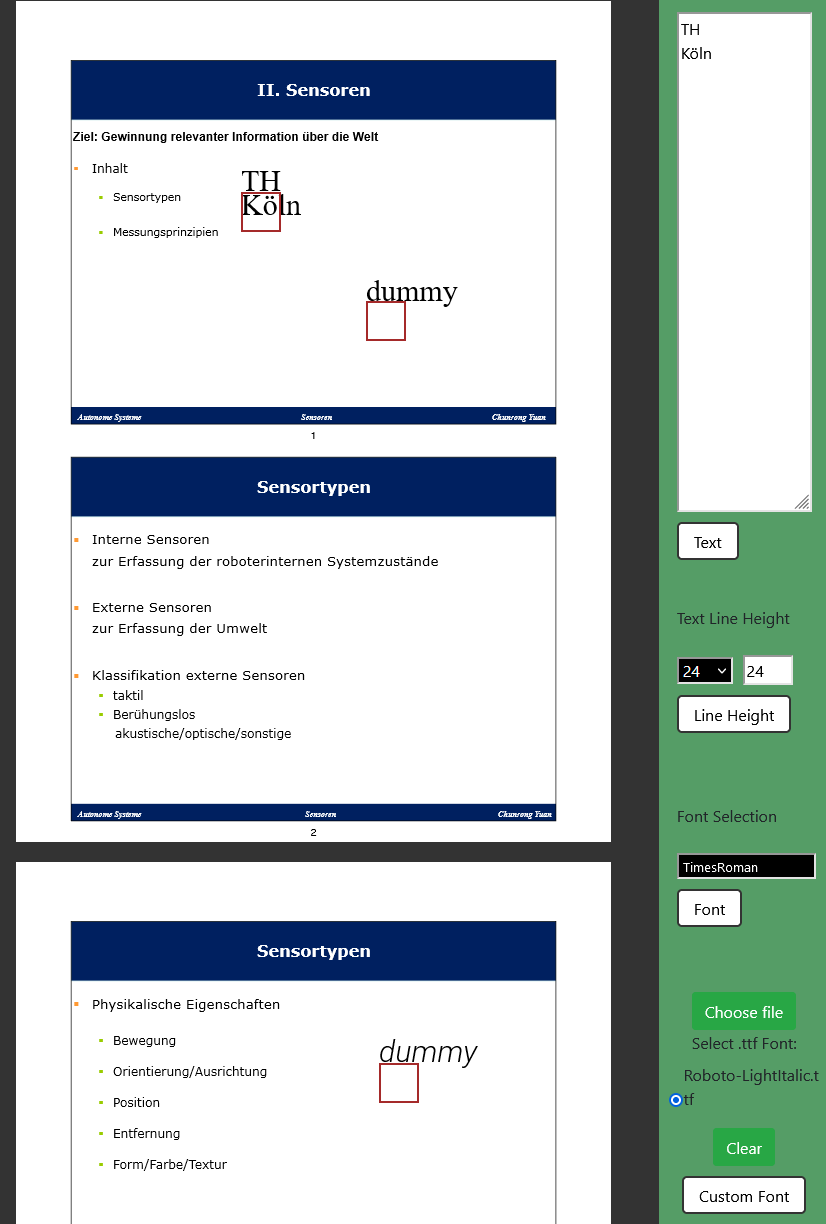
\includegraphics[width=1\textwidth]{"images/texteditor3.png"}
	\caption{Modifizierter Text im Texteditor der PDF Web App}
	\label{fig:texteditor3}
\end{figure}

\begin{figure}[!htbp]
	\centering
	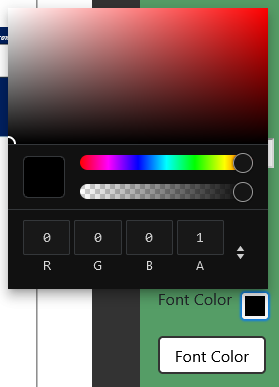
\includegraphics[width=0.6\textwidth]{"images/fontcolor.png"}
	\caption{Color picker für die Fontfarbe des Texteditors der PDF Web App}
	\label{fig:fontcolor}
\end{figure}